\documentclass{article}
\usepackage[margin=1in]{geometry}
\usepackage{amsmath,amsthm,amssymb}
\usepackage{bbm,enumerate,mathtools}
\usepackage{tikz,pgfplots}
\usepackage{chessboard}
\usepackage[hidelinks]{hyperref}
\usepackage{multicol} % Problem 35
\usepackage{xstring} % Difficulty command
\usetikzlibrary{shapes.geometric}

\newenvironment{question}{\begin{trivlist}\item[\textbf{Question.}]}{\end{trivlist}}
\newenvironment{note}{\begin{trivlist}\item[\textbf{Note.}]}{\end{trivlist}}
\newenvironment{references}{\begin{trivlist}\item[\textbf{References.}]}{\end{trivlist}}
\newenvironment{related}{\begin{trivlist}\item[\textbf{Related.}]\end{trivlist}\begin{enumerate}}{\end{enumerate}}

\newcommand\score[1]{
\pgfmathsetmacro\pgfxa{#1+1}
\tikzstyle{scorestars}=[
  star,
  star points=5,
  star point ratio=2.25,
  draw,
  inner sep=3pt,
  anchor=outer point 5
]
  \begin{tikzpicture}[baseline]
    \draw[opacity=0] (0,-0.5) rectangle (0,0.2); % Workaround for whitespace at the bottom.
    \foreach \i in {1,...,4} {
      \pgfmathparse{(\i<=#1?"yellow":"gray")}
      \edef\starcolor{\pgfmathresult}
      \draw (\i*4.5ex,0) node[name=star\i,scorestars,fill=\starcolor]  {};
    }
  \end{tikzpicture}
}

\newcommand{\difficulty}[1]{%
  \IfEqCase{#1}{%
      {1}{
        
\begin{tikzpicture}[scale=0.7, baseline=0.9mm]%
          \definecolor{slopegreen}{rgb}{0.0, 0.5, 0.0}%
          \fill[slopegreen] (0.5,0.5) circle (0.5);%
        \end{tikzpicture}%
      }%
      {2}{
        
\begin{tikzpicture}[scale=0.7, baseline=0.9mm]%
          \definecolor{slopeblue}{rgb}{0.0, 0.44, 1.00}
          \fill[slopeblue] (0,0) rectangle (1,1);%
        \end{tikzpicture}%
      }%
      {3}{
\begin{tikzpicture}[scale=0.7, baseline=0.9mm]\fill (0,0.5)--(0.5, 0)--(1,0.5)--(0.5,1)--cycle; \end{tikzpicture}}%
      {4}{
\begin{tikzpicture}[scale=0.7, baseline=0.9mm]\fill (0.25,0)--(0,0.5)--(0.25,1)--(0.5,0.5)--cycle; \fill (0.75,0)--(0.5,0.5)--(0.75,1)--(1,0.5)--cycle;\end{tikzpicture}}%
      % you can add more cases here as desired
  }[\PackageError{difficulty}{Undefined difficulty level: #1}{}]%
}%
\newcommand{\rating}[2]{\difficulty{#1}\\\score{#2}\\}


\begin{document}
\rating{2}{2}
In the ``nine dots puzzle'' or ``thinking outside the box puzzle'', a player is
asked to connect dots arranged in a $3 \times 3$ grid using four lines.
This can be generalized to connecting the dots of a $n \times n$ grid with
$2n - 2$ lines.
\begin{figure}[ht!]
  \centering
  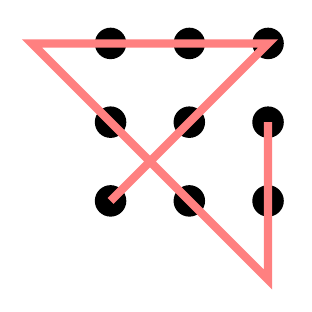
\begin{tikzpicture}
    \foreach \x in {1,2,3} {
      \foreach \y in {1,2,3} {
        \fill (\x, \y) circle (0.2);
      }
    }
    \draw[red!50, line width=3] (1,1)--(3,3)--(0,3)--(3,0)--(3,2);
  \end{tikzpicture}
  \\~\\
  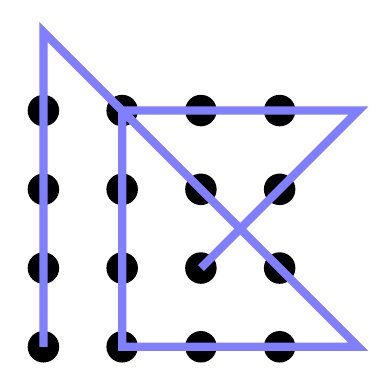
\begin{tikzpicture}
    \foreach \x in {1,...,4} {
      \foreach \y in {1,...,4} {
        \fill (\x, \y) circle (0.2);
      }
    }
    \draw[blue!50, line width=3] (1,1)--(1,5)--(5,1)--(2,1)--(2,4)--(5,4)--(3,2);
  \end{tikzpicture}
  \hspace{1cm}
  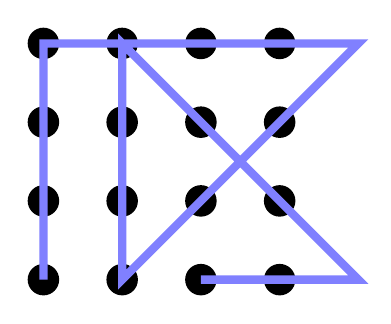
\begin{tikzpicture}
    \foreach \x in {1,...,4} {
      \foreach \y in {1,...,4} { \fill (\x, \y) circle (0.2); }
    }
    \draw[blue!50, line width=3] (1,1)--(1,4)--(5,4)--(2,1)--(2,4)--(5,1)--(3,1);
  \end{tikzpicture}
  \hspace{1cm}
  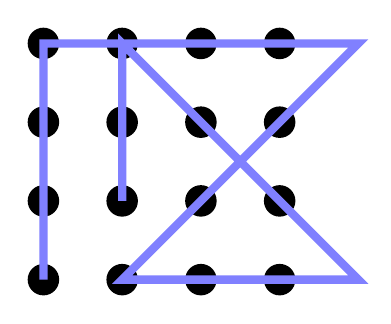
\begin{tikzpicture}
    \foreach \x in {1,...,4} {
      \foreach \y in {1,...,4} { \fill (\x, \y) circle (0.2); }
    }
    \draw[blue!50, line width=3] (1,1)--(1,4)--(5,4)--(2,1)--(5,1)--(2,4)--(2,2);
  \end{tikzpicture}
  \caption{
    The unique (?) way of completing the $3 \times 3$ grid,
    and three distinct ways of completing the $4 \times 4$ grid.
  }
\end{figure}
\begin{question}
  How many distinct solutions exist on the $n \times n$ grid?
\end{question}

\begin{related}
  \item What if you want to minimize the area ``outside'' of the grid?
  \item What if you must start and end from the same point?
  \item What if you want to minimize the path length?
  \item Do any of these have lines that aren't horizontal, vertical, or $45^\circ$ diagonal?
  \item What if this is done on other figures? (Triangles, Diamonds, Octagons, Stars, etc.)
  \item Can this be generalized into higher dimensions with lines? Hyperplanes?
  \item What if the ``pencil'' can be lifted $k \geq 1$ times?
  \item What if this is done on a torus or cylinder?
\end{related}
\begin{references}
  \item \url{https://math.stackexchange.com/q/21851/121988}
  \item \url{https://en.wikipedia.org/wiki/Thinking_outside_the_box#Nine_dots_puzzle}
  \item \href{https://chalkdustmagazine.com/features/thinking-outside-outside-box/}{Thinking outside outside the box} by Rob Eastaway
\end{references}
\end{document}
